\begin{exercise}
The value of an action, $q_\pi(s, a)$, depends on the expected next reward and the expected sum of the remaining rewards.
Again we can think of this in terms of a small backup diagram, this one rooted at an action (state-action pair) and branching to the possible next states:

\begin{figure}[H]
    \centering
    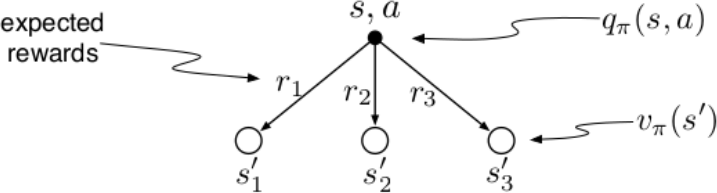
\includegraphics[width = 0.5 \textwidth]{2.19.png}
    \caption{}
    \label{fig:2.19}
\end{figure}

Give the equation corresponding to this intuition and diagram for the action value, $q_\pi(s, a)$, in terms of the expected next reward, $R_{t+1}$ , and the expected next state value, $v_\pi(S_{t+1})$, given that $S_t = s$ and $A_t = a$.
This equation should include an expectation but not one conditioned on following the policy.
Then give a second equation, writing out the expected value explicitly in terms of $p(s_0, r \mid s, a)$ defined by \eqref{eq:2.13}, such that no expected value notation appears in the equation.

\end{exercise}

\begin{solution}
With the law of total expectation we get:

\begin{align*}
  q_\pi(s,a)
  &=
  \E_\pi\big[G_t\mid S_t = s, A_t = a\big]
  =
  \E_\pi\big[R_{t+1} + G_{t+1}\mid S_t = s, A_t = a\big] \\
  &=
  \sum_{r,s^\prime} p(s^\prime, r\mid s,a) \E_\pi\big[R_{t+1} + G_{t+1}\mid S_t = s, A_t = a, S_{t+1} = s^\prime, R_{t+1} = r\big] \\
  &=
  \sum_{r,s^\prime} p(s^\prime, r\mid s,a)\Big[r + \gamma \E_\pi\big[G_{t+1}\mid S_{t+1} = s^\prime\big] \Big]\\
  &=
  \sum_{r,s^\prime} p(s^\prime, r\mid s,a)\Big[r + \gamma v_\pi(s^\prime)\Big]
  =
  \E\big[R_{t+1} + v_\pi(S_{t+1})\mid S_t = s, A_t = a\big]
\end{align*}

\end{solution}
